\documentclass[aps,prl,reprint,superscriptaddress, longbibliography]{revtex4-1}
\usepackage{H1}
\usepackage[pdftex,colorlinks=true]{hyperref}
\hypersetup{citecolor = blue}
\usepackage[normalem]{ulem}
\usepackage{color}
\usepackage[usenames,dvipsnames,svgnames,table]{xcolor}
\usepackage{mathtools}
\usepackage{enumerate}

\newcommand{\vedika}[1]{ {\color{red} {{#1}}}}
\newcommand{\david}[1]{ {\color{blue} {{#1}}}}
\newcommand{\charlie}[1]{ {\color{Magenta} {{#1}}}}

\newcommand{\Tr}{ \mbox{Tr}}
\newcommand{\vb}{v_B}
\newcommand{\I}{\mathbb{I}}
\newcommand{\ip}{i+1}
\newcommand{\mc}[1]{ { \mathcal {{#1}}}}
\newcommand{\Sz}{S_z^{\rm tot}}
\newcommand{\lamv}{\lambda(v)}
\newcommand{\otoc}{{C}({\bf x},t)}

\begin{document}
\title{Asymmetric butterfly velocities in local\\ time-independent Hamiltonians
} 
%
%\author{Charles Stahl}
%\affiliation{\mbox{Department of Physics, Princeton University, Princeton, NJ 08544, USA}}
%\affiliation{\mbox{DAMTP}}
%\author{Vedika Khemani}
%\affiliation{\mbox{Department of Physics, Harvard University, Cambridge, MA 02138, USA}}
%\author{David A. Huse}
%\affiliation{\mbox{Department of Physics, Princeton University, Princeton, NJ 08544, USA}}

\begin{abstract}
The butterfly velocity $v_B$ is the velocity at which initially local operators spread. In many 1-D systems this velocity is independent of the direction of spreading. This need not be the case. In fact, with arbitrarily nonlocal Hamiltonians, or arbitrarily deep circuit models, the ratio of the two butterfly velocities may be made arbitrarily large. We provide a class of circuits whose limiting behavior shows this arbitrarily large ratio. We also describe a local Hamiltonian with an asymmetric $v_B$, presenting various methods to measure the asymmetry.
\end{abstract}

\maketitle

\section{Introduction}

Thermalization is important because\dots

Asymmetric transport is seen in ``staircase" and ``glider" circuits, but we wanted to show it is also possible in time-independent Hamiltonians. 

\begin{figure}
	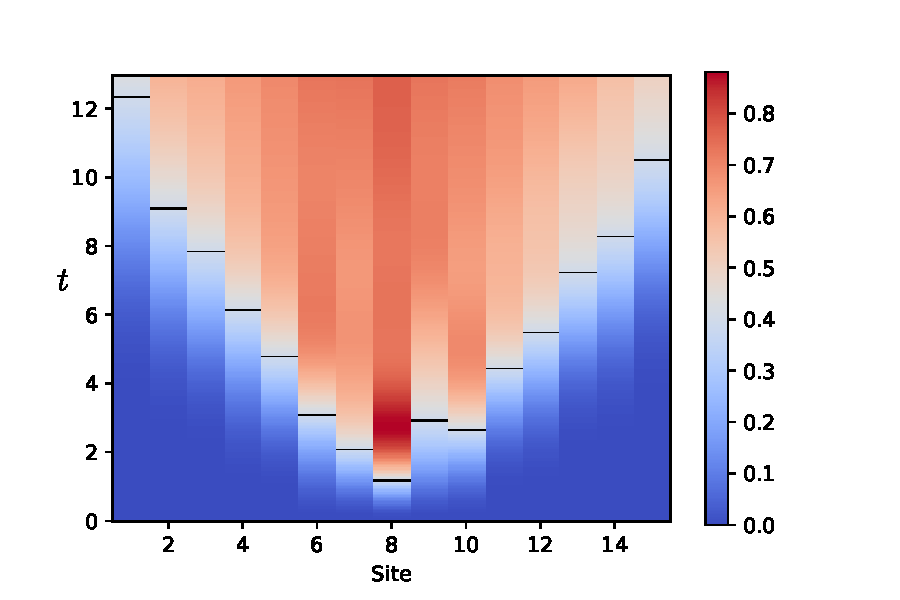
\includegraphics[width=\columnwidth]{colorplot}
	\caption{Illustration of the initially local operator. The bars indicate the time at which the OTOC passes 0.4, to emphasize the asymmetry.}
	\label{fig:colorplot}
\end{figure}

In this paper we will\dots

\pagebreak

\section{Circuit models with asymmetric $v_B$} \label{sec:circ}

In a 1-D circuit, how asymmetric can the spreading be?

On the edge of a 2-D system, spreading can be chiral even with a finite circuit depth~\cite{PoChiralCircuit}.

To be completely chiral with only 1 dimension, the circuit will have to be of infinite depth.

Given a constraint on the depth, how asymmetric can the spreading be?

\charlie{How much of the circuit model, with $\Gamma(ds/dx)$, etc. should we describe here?}

For the growth rate curves of $n$-stair circuits for $n\le 6$ see Fig.~\ref{fig:compareRates}.

\begin{figure}
	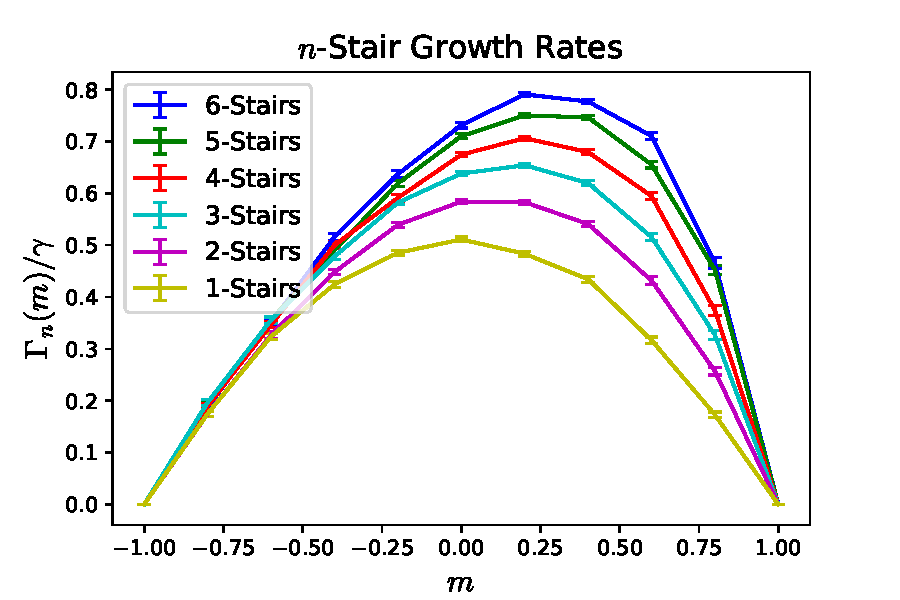
\includegraphics[width=\columnwidth]{compareRates.pdf}
	\caption{Empirical growth rate as a function of slope for $n$-stair circuits. The right/forward and left/backward butterfly velocities are the slopes of these curves at their endpoint, indicating that as the left $v_B$ stays constant, the right $v_B$ increases. The appendix includes an argument that the right $v_B$ is unbounded in the large-$n$ limit.}
	\label{fig:compareRates}
\end{figure}	

For small $n$, we can simulate the circuit directly. This is particularly easy in the large $q$ limit, where $q$ is the dimension of the Hilbert space at each site. \charlie{Again, how in-depth should this section be?}.

For large $n$, approaching the size of the system, we can approximate the entanglement curve as being uncorrelated. In that limit, the growth rate is $\Gamma(ds/dt) = ds/dt+1$, so that for spreading to the left $v_B=1$ and for spreading to the right $v_B=\infty$.

\section{Local Hamiltonians}

Motivate triple product:
Has to be asymmetric-can't have 2-site interactions.
Impose SU(2) as a constraint?
Then our only option is the triple product.

Alone, this model is not general.
Large degeneracy at $E=0$. 
Explain the degeneracy is due to the $E\to -E$ (anti-)symmetry.
Show parts of this degeneracy can be broken with various fields.
A random $Z$ field breaks all the degeneracy.
This phase change can be seen in Fig.~\ref{fig:levelrepultrans}.

\begin{figure}
	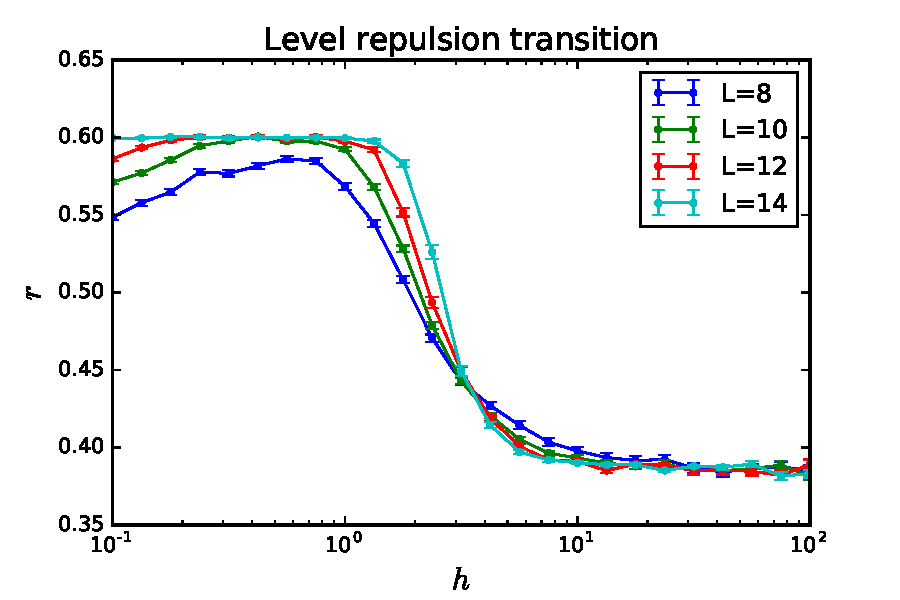
\includegraphics[width=\columnwidth]{levelrepultrans}
	\caption{Phase transition for the model, with level repulsion parameter plotted against field strength. Note that in the thermalizing phase the ratio is $~0.6$ instead of $0.53$ because the statistics are GUE instead of GOE. \charlie{I think I remember Vedika saying this but I can't find where.}}
	\label{fig:levelrepultrans}
\end{figure}

We will measure the asymmetry using two metrics. The first is the weight of all operators with right (left) endpoint on site $i$, which we will call the right (left) weight. The other is the OTOC. \charlie{should we define these in this section?} \charlie{Make sure to point out use of initial operators as being on site 0 or $L-1$}.

In the thermalizing, generic phase, the right weights peak as the information front passes. Because of the three-site nature of each term in the Hamiltonian, the right weight and OTOC exhibit an ``odd-even" effect. It is possible to account for these by averaging judiciously, or by only looking at even (or odd) sites. At $L=13$, there are enough even sites that the asymmetry can be seen. For a picture of the rights weights with their successive peaks, see Fig.~\ref{fig:Rweightpeakshape}. 

\begin{figure}
	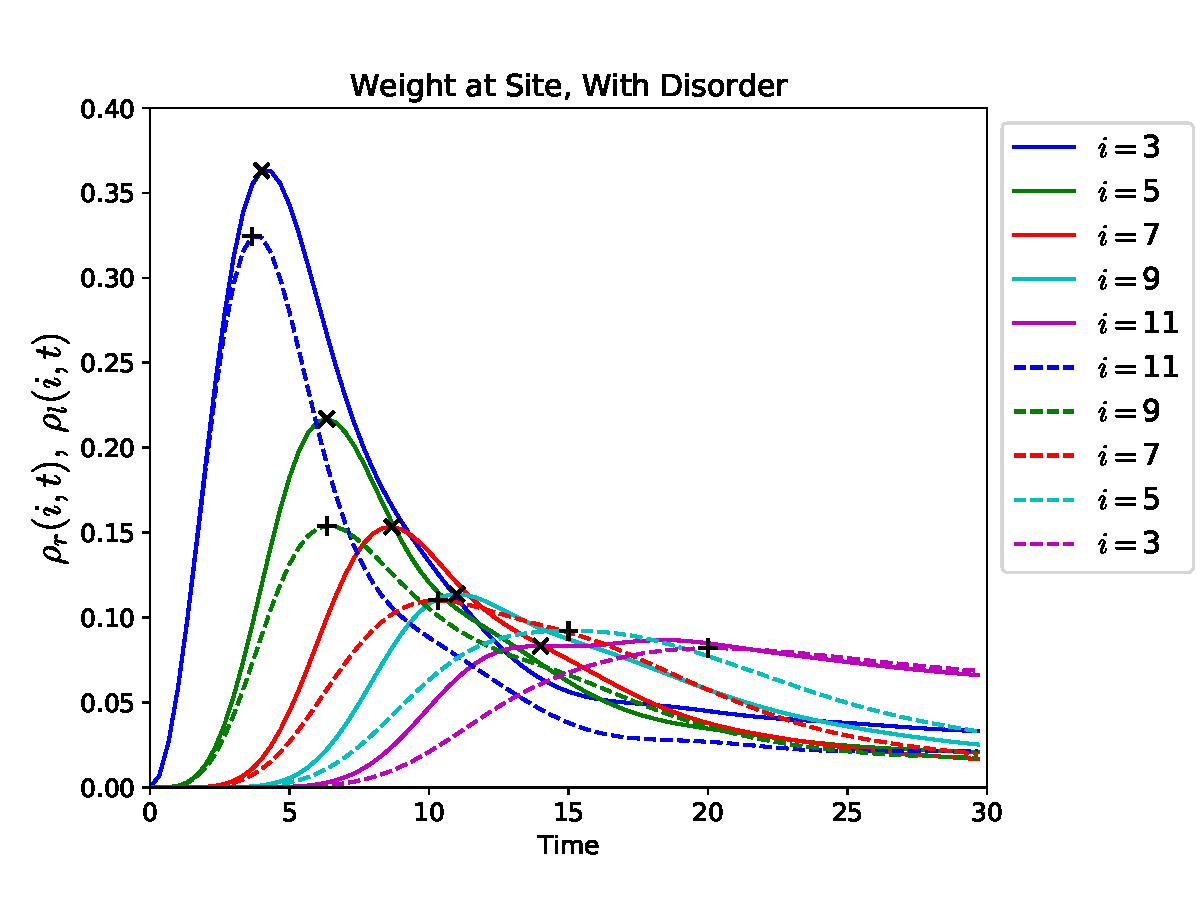
\includegraphics[width=\columnwidth]{Rweightpeakshape}
	\caption{Right weight at even sites for $L=13$. The peak travels ballistically. Later peaks are smaller \charlie{Is this due to broadening?}}
	\label{fig:Rweightpeakshape}
\end{figure}

Fig.~\ref{fig:Rweightpeaktimes} shows the peaks traveling ballistically. The peaks reach equivalent sites at later times for the left-moving wave, implying $v_{B,l}<v_{B,r}$. We can extract $v_{B,l}$ and $v_{B,r}$ from these curves by fitting linear functions to the peak timings.

\begin{figure}
	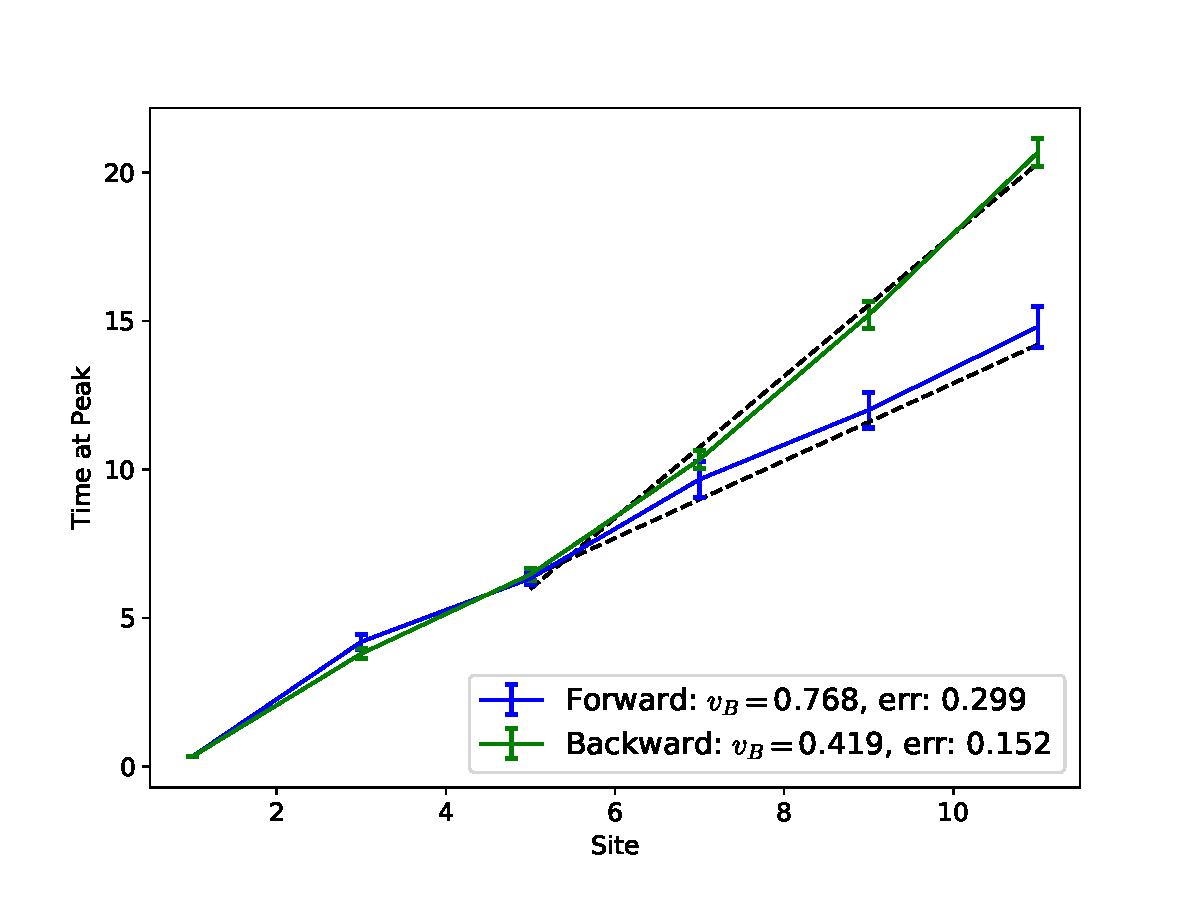
\includegraphics[width=\columnwidth]{Rweightpeaktimes}
	\caption{Time of peak vs. site. Since this is plot of time as a function of distance, the larger slope in the left weight means that $v_B$ is larger for propagation to the right. \charlie{This has the wrong normalization but I'm working on it.}}
	\label{fig:Rweightpeaktimes}
\end{figure}

It is also possible to extract butterfly velocities from the the velocity-dependent Lyapunov exponents. Fig.~\ref{fig:vdle} shows the VDLEs for the right-going and left-going OTOCs. $v_B$ is defined by $\lambda(v_B) = 0$, so the plot shows that $v_{B,r}>v_{B,l}$.

\begin{figure}
	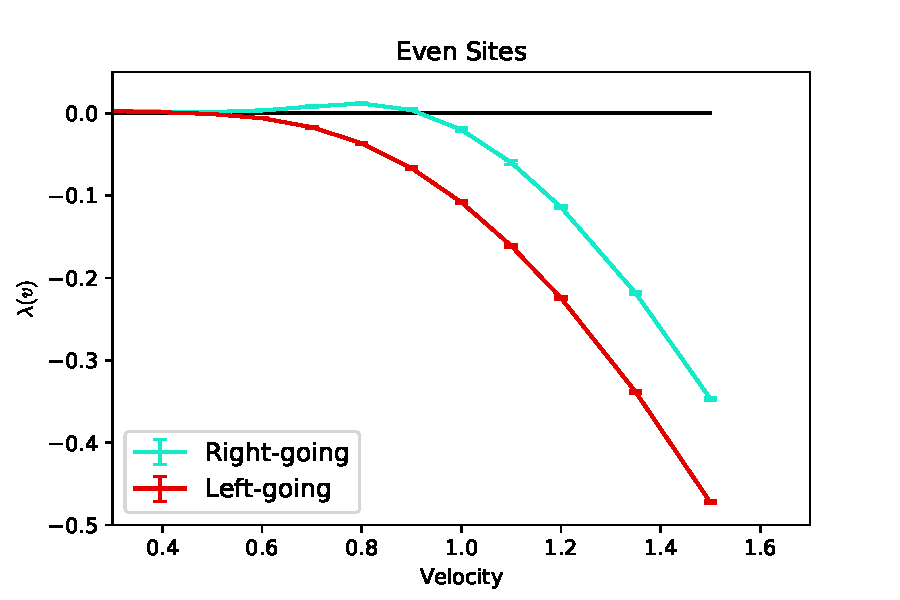
\includegraphics[width=\columnwidth]{vdle}
	\caption{Velocity-dependent Lyapunov exponents extracted from the OTOC on even sites. Since $\lambda_r(v)>\lambda_l(v)$, we know $v_{B,r}>v_{B,l}$.}
	\label{fig:vdle}
\end{figure}

\section{Conclusion}

Advantages of this model:
Time-independent Hamiltonian.
Only ingredients are chains of two-level systems.

Further work:
How do the velocities depend on $h$?
What happens at the phase transition?
Maximally asymmetric three-site Hamiltonians?
2-D systems?

%We'll want to cite a bunch of people~\cite{Larkinotoc,Lieb72,KitaevSYK,chaosbound,HosurYoshida,ShenkerStanfordButterfly,LocalizedShocks,CotlerRM,RobertsStanford,GuQiStanford,GuQi_rcft,StanfordWeakCoupling,PatelDiffusiveMetal,ChowdhuryON,Galitski_lyapunov,DoraMoessner,LuitzScrambling,ProsenWeakChaos,AleinerOTOC,MotrunichTFIM_otoc,FradkinHuse,ChalkerFloquetChaos,FawziScrambling,opspreadAdam, opspreadCurt, TiborCons, KhemaniCons}.

\section*{Acknowledgements}
We thank many people.

\charlie{Note somewhere about arXiv:1809.02614v1}

\bibliography{global}

\begin{appendix}


\end{appendix}

\end{document}
